\section{Ramanujanovi grafi}
Koncept ramanujanovih grafov ima preprosto definicijo, vendar njen pomen ni očiten brez predhodne motivacije s sorodnimi definicijami in izreki. Te nam razjasnijo povezavo med lastnimi vrednostmi grafa, ki se pojavijo v definiciji Ramanujanovih grafov, ter povezljivostjo grafa.
\subsection{Cheegerjeva konstanta}
Kot v uvodnem primeru nas zanima koliko povezav moramo odstraniti, da graf ni več povezan.

Naj bo \(G=(V,E)\) povezan graf in \(S\subseteq V\) podmnožica vozlišč z \(0<\abs{S} \leq \abs{V}/{2}\). Z \(\partial S\subseteq E\) označimo množico povezav od \(S\) do komplementa vozlišč, \(\overline{S}\). Če iz grafa odstranimo \(\partial S\), potem se graf razdeli na več komponent.

Največjo težavo predstavljajo ozka grla grafa. To je majhna množica povezav, ki ločuje dva dela grafa z velikim številom vozlišč. Da je graf dobro povezan torej želimo, da ni ozkih grl in da je za velik \(\abs{S}\) tudi velik \(\abs{\partial S} \), oziroma da \(\abs{S}/{\abs{\partial S}}\) ni nikoli majhen.

\begin{definicija}[Cheegerjeva konstanta]
    Za graf \(G = (V,E)\) in podmnožice njegovih vozlišč 
    \begin{align*}
        T = \left\{S\subseteq V \mid 0<\abs{S} \leq \frac{\abs{V}}{2}\right\}    
    \end{align*}
    definiramo Cheegerjevo konstanto \cite{polatajko} kot
    \begin{align*}
        c(G) = \min_{S\in T} \frac{\abs{\partial S}}{\abs{S}}
    \end{align*}
\end{definicija}
Večja kot je vrednost \(c(G)\), manj ozkih grl ima graf \(G\).

\begin{primer}[Cikli]
    \hspace{0em}
    \begin{center}
        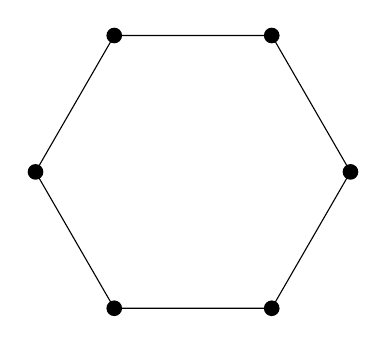
\begin{tikzpicture}
            % Defining the vertices of the cycle
            \foreach \x in {0,60,...,300} {
                    \node[circle, fill=black, inner sep=2pt] at (\x:2) {};
                }
            % Drawing the edges of the cycle
            \draw (0:2) -- (60:2) -- (120:2) -- (180:2) -- (240:2) -- (300:2) -- cycle;
        \end{tikzpicture}
    \end{center}

    Za minimizacijo izraza \(\abs{\partial S}/{\abs{S}}\) lahko izberemo množico sosednjih vozlišč. Tako bo vedno \(\abs{\partial S} = 2\), \(S\) pa povečamo do polovice cikla, kot omejuje definicija. Za cikel \(C_{2n}\) torej vzamemo \(\abs{S} = n\), za \(C_{2n+1}\) pa prav tako \(\abs{S} = n\).
    \begin{align*}
        c(C_n) = \frac{2}{\lfloor \frac n2\rfloor}
    \end{align*}
    Večji kot je \(n\), manjša je Cheegerjeva konstanta, kar pomeni, da je graf slabše povezan, saj je potrebno odstraniti le dve povezavi, da ločimo graf na dve veliki komponenti.
\end{primer}
\begin{primer}[Polni grafi]
    \hspace{0em}
    \begin{center}
        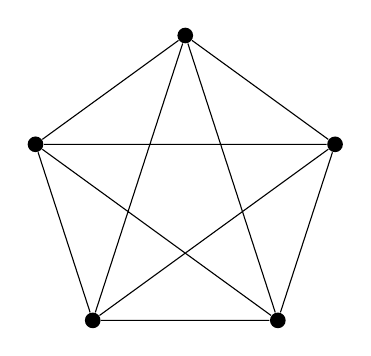
\begin{tikzpicture}
            \node[circle, fill=black, inner sep=2pt] (A) at (90:2) {};
            \node[circle, fill=black, inner sep=2pt] (B) at (162:2) {};
            \node[circle, fill=black, inner sep=2pt] (C) at (234:2) {};
            \node[circle, fill=black, inner sep=2pt] (D) at (306:2) {};
            \node[circle, fill=black, inner sep=2pt] (E) at (18:2) {};
            \draw (A) -- (B) -- (C) -- (D) -- (E) -- (A);
            \draw (A) -- (C) -- (E) -- (B) -- (D) -- (A);
        \end{tikzpicture}
    \end{center}
    Za poln graf \(K_n\) velja, da je \(\abs{\partial S} = \abs{S} \cdot (n - \abs{S})\). Zato je
    \begin{align*}
        c(K_n) = \min_{S} n-\abs{S}.
    \end{align*}
    Minimum dosežemo pri \(\abs{S} = \lfloor\frac n2\rfloor\) s poljubno izbiro vozlišč.
    \begin{align*}
        c(K_n) = \left\lceil \frac n2 \right\rceil
    \end{align*}
    Večji kot je \(n\), večja je Cheegerjeva konstanta in graf je bolje povezan.
\end{primer}
Oglejmo si primer, kjer je zelo očitna povezava med ozkim grlom grafa in Cheegerjevo konstanto.
\begin{primer}[Ozko grlo]\label{ozko-grlo-cheeger}\hspace{0em}
    \begin{figure}[H]
        \centering
        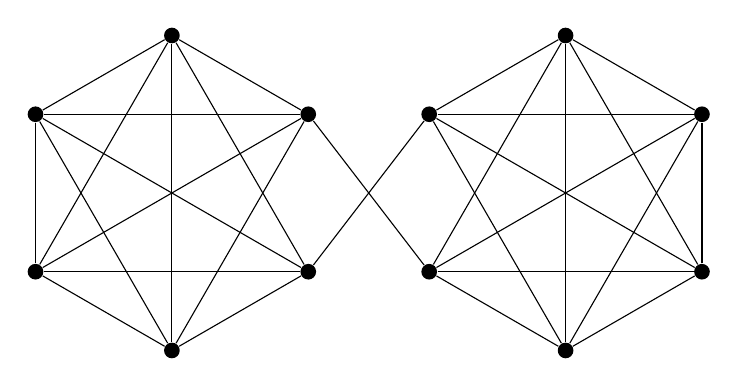
\begin{tikzpicture}
            % First K_5
            \begin{scope}[shift={(0,0)}]
                \node[circle, fill=black, inner sep=2pt] (A1) at (90:2)  {};
                \node[circle, fill=black, inner sep=2pt] (B1) at (150:2) {};
                \node[circle, fill=black, inner sep=2pt] (C1) at (210:2) {};
                \node[circle, fill=black, inner sep=2pt] (D1) at (270:2) {};
                \node[circle, fill=black, inner sep=2pt] (E1) at (330:2) {};
                \node[circle, fill=black, inner sep=2pt] (F1) at (30:2)  {};
                \draw (A1) -- (B1);
                \draw (A1) -- (C1);
                \draw (A1) -- (D1);
                \draw (A1) -- (E1);
                \draw (A1) -- (F1);
                \draw (B1) -- (C1);
                \draw (B1) -- (D1);
                \draw (B1) -- (E1);
                \draw (B1) -- (F1);
                \draw (C1) -- (D1);
                \draw (C1) -- (E1);
                \draw (C1) -- (F1);
                \draw (D1) -- (E1);
                \draw (D1) -- (F1);
            \end{scope}

            % Second K_5
            \begin{scope}[shift={(5,0)}]
                \node[circle, fill=black, inner sep=2pt] (A2) at (90:2) {};
                \node[circle, fill=black, inner sep=2pt] (B2) at (150:2) {};
                \node[circle, fill=black, inner sep=2pt] (C2) at (210:2) {};
                \node[circle, fill=black, inner sep=2pt] (D2) at (270:2) {};
                \node[circle, fill=black, inner sep=2pt] (E2) at (330:2) {};
                \node[circle, fill=black, inner sep=2pt] (F2) at (30:2) {};
                \draw (A2) -- (B2);
                \draw (A2) -- (C2);
                \draw (A2) -- (D2);
                \draw (A2) -- (E2);
                \draw (A2) -- (F2);
                \draw (B2) -- (D2);
                \draw (B2) -- (E2);
                \draw (B2) -- (F2);
                \draw (C2) -- (D2);
                \draw (C2) -- (E2);
                \draw (C2) -- (F2);
                \draw (D2) -- (E2);
                \draw (D2) -- (F2);
                \draw (E2) -- (F2);
            \end{scope}

            % Connecting edge between the two K_6 graphs
            \draw (F1) -- (C2);
            \draw (E1) -- (B2);
        \end{tikzpicture}
        \caption{Povezana grafa \(K_6\)}
    \end{figure}
    Za \(n\geq3\) vzamemo dva polna grafa \(K_n\) in pri vsakemu izberemo dve vozlišči. Dobimo vozlišči \(u_1, v_1\) prvega grafa in \(u_2, v_2\) drugega grafa. Odstranimo povezavi \((u_1, v_1)\) in \((u_2, v_2)\) in dodamo \((u_1, v_2)\), \((u_2, v_1)\), da tvorimo regularen povezan graf \(G = (V,E)\). Če za \(S\) vzamemo enega izmed polnih grafov, je \(\abs{S} = n\) maksimalen in \(\abs{\partial S} = 2\) minimalen. Torej je Cheegerjeva konstanta
    \begin{align*}
        c(G) = \frac{2}{n}.
    \end{align*}
    Večji kot je \(n\), bolj izrazito je ozko grlo na grafu, kar vidimo tudi v manjši vrednosti \(c(G)\). V primeru \(n=6\) smo dobili 5-regularen graf na dvanajstih vozliščih s \(c(G)=0.4\).
\end{primer}
Če izberemo naključen graf pa je verjetnost, da ima ozko grlo majhna. Oglejmo si primer naključno izbranega \(5\)-regularnega grafa na dvanajstih vozliščih.
% [[0. 0. 1. 1. 1. 0. 0. 0. 0. 1. 0. 1.]
%  [0. 0. 1. 0. 1. 1. 0. 1. 0. 0. 0. 1.]
%  [1. 1. 0. 0. 1. 1. 0. 1. 0. 0. 0. 0.]
%  [1. 0. 0. 0. 0. 1. 0. 1. 1. 0. 1. 0.]
%  [1. 1. 1. 0. 0. 0. 0. 0. 1. 0. 1. 0.]
%  [0. 1. 1. 1. 0. 0. 1. 0. 0. 0. 0. 1.]
%  [0. 0. 0. 0. 0. 1. 0. 1. 1. 1. 0. 1.]
%  [0. 1. 1. 1. 0. 0. 1. 0. 0. 1. 0. 0.]
%  [0. 0. 0. 1. 1. 0. 1. 0. 0. 1. 1. 0.]
%  [1. 0. 0. 0. 0. 0. 1. 1. 1. 0. 1. 0.]
%  [0. 0. 0. 1. 1. 0. 0. 0. 1. 1. 0. 1.]
%  [1. 1. 0. 0. 0. 1. 1. 0. 0. 0. 1. 0.]]
% To be ramanujan, ev under 4.0
% Spectral gap 1.503064554001702
% Eigenvalue: 3.4969354459982944
% Is ramanujan:  True
% [0, 3, 4, 8, 9, 10]
% Cheeger: 1.6666666666666667
\begin{primer}[Naključen graf]\label{nakljucen-graf-cheeger}
    Naj bo \(G\) graf s sosednostno matriko
    \begin{align*}
        A = \begin{bmatrix}
            0 & 0& 1& 1& 1& 0& 0& 0& 0& 1& 0 &1\\
            0 & 0& 1& 0& 1& 1& 0& 1& 0& 0& 0 &1\\
            1 & 1& 0& 0& 1& 1& 0& 1& 0& 0& 0 &0\\
            1 & 0& 0& 0& 0& 1& 0& 1& 1& 0& 1 &0\\
            1 & 1& 1& 0& 0& 0& 0& 0& 1& 0& 1 &0\\
            0 & 1& 1& 1& 0& 0& 1& 0& 0& 0& 0 &1\\
            0 & 0& 0& 0& 0& 1& 0& 1& 1& 1& 0 &1\\
            0 & 1& 1& 1& 0& 0& 1& 0& 0& 1& 0 &0\\
            0 & 0& 0& 1& 1& 0& 1& 0& 0& 1& 1 &0\\
            1 & 0& 0& 0& 0& 0& 1& 1& 1& 0& 1 &0\\
            0 & 0& 0& 1& 1& 0& 0& 0& 1& 1& 0 &1\\
            1 & 1& 0& 0& 0& 1& 1& 0& 0& 0& 1 &0\\
        \end{bmatrix}.
    \end{align*}
    Graf smo izbrali enakomerno naključno izmed vseh 5-regularnih grafov na dvanajstih vozliščih.
    \begin{figure}[H]
        \centering
        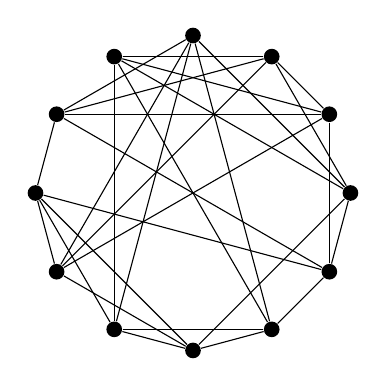
\begin{tikzpicture}
            \node[circle, fill=black, inner sep=2pt] (A) at (0.0: 2) {};
            \node[circle, fill=black, inner sep=2pt] (B) at (30.0: 2) {};
            \node[circle, fill=black, inner sep=2pt] (C) at (60.0: 2) {};
            \node[circle, fill=black, inner sep=2pt] (D) at (90.0: 2) {};
            \node[circle, fill=black, inner sep=2pt] (E) at (120.0: 2) {};
            \node[circle, fill=black, inner sep=2pt] (F) at (150.0: 2) {};
            \node[circle, fill=black, inner sep=2pt] (G) at (180.0: 2) {};
            \node[circle, fill=black, inner sep=2pt] (H) at (210.0: 2) {};
            \node[circle, fill=black, inner sep=2pt] (I) at (240.0: 2) {};
            \node[circle, fill=black, inner sep=2pt] (J) at (270.0: 2) {};
            \node[circle, fill=black, inner sep=2pt] (K) at (300.0: 2) {};
            \node[circle, fill=black, inner sep=2pt] (L) at (330.0: 2) {};
            \draw (C) -- (A);
            \draw (C) -- (B);
            \draw (D) -- (A);
            \draw (E) -- (A);
            \draw (E) -- (B);
            \draw (E) -- (C);
            \draw (F) -- (B);
            \draw (F) -- (C);
            \draw (F) -- (D);
            \draw (G) -- (F);
            \draw (H) -- (B);
            \draw (H) -- (C);
            \draw (H) -- (D);
            \draw (H) -- (G);
            \draw (I) -- (D);
            \draw (I) -- (E);
            \draw (I) -- (G);
            \draw (J) -- (A);
            \draw (J) -- (G);
            \draw (J) -- (H);
            \draw (J) -- (I);
            \draw (K) -- (D);
            \draw (K) -- (E);
            \draw (K) -- (I);
            \draw (K) -- (J);
            \draw (L) -- (A);
            \draw (L) -- (B);
            \draw (L) -- (F);
            \draw (L) -- (G);
            \draw (L) -- (K);
        \end{tikzpicture}
        \caption{Naključno izbran graf.}
    \end{figure}
    Za graf s pomočjo računalnika izračunamo Cheegerjevo konstanto tako, da preverimo vse možne izbire \(S \subset \{1, \ldots, 12\}\). V tem primeru je optimalna izbira \(S = \{1, 4, 5, 9, 10, 11\}\) in Cheegerjeva konstanta je \(c(G)\approx 1.66\), veliko višje kot v primeru grafa z ozkim grlom, kljub temu, da sta imela enako stopnjo regularnosti in enako število vozlišč.
\end{primer}
\subsection{Spektralna vrzel}
Sedaj se namesto geometrijskih lastnosti grafov osredotočimo na njihove algebraične lastnosti. Vsak graf lahko identificiramo z njegovo sosednostno matriko, ki je simetrična matrika z elementi 0 in 1. Po spektralnem izreku ima torej \(n\) realnih lastnih vrednosti \(\lambda_i\), ki jih lahko uredimo po velikosti.
\begin{align*}
    \lambda_1 \geq \lambda_2 \geq \ldots \geq \lambda_n
\end{align*}

\begin{definicija}[Spektralna vrzel]
    Spektralna vrzel grafa \(G\) je razlika med največjo in drugo največjo lastno vrednostjo njegove sosednostne matrike.
    \begin{align*}
        s(G) = \lambda_1 - \lambda_2
    \end{align*}
\end{definicija}
\begin{primer}[Cikli]
    Graf \(C_n\) ima sosednostno matriko
    \begin{align*}
        N(C_n) = \begin{bmatrix}
                     0      & 1      & 0      & 0      & \cdots & 0      & 0      & 1      \\
                     1      & 0      & 1      & 0      & \cdots & 0      & 0      & 0      \\
                     0      & 1      & 0      & 1      & \cdots & 0      & 0      & 0      \\
                     \vdots & \vdots & \vdots & \vdots & \ddots & \vdots & \vdots & \vdots \\
                     0      & 0      & 0      & 0      & \cdots & 1      & 0      & 1
                 \end{bmatrix}.
    \end{align*}
    Matrika je cirkulantna, zato poznamo njene lastne vrednosti \cite{circulant}.
    \begin{align*}
        \lambda(N(C_n)) = \left\{ 2 \cos\left(\frac{2\pi k}{n}\right) \mid 0 \leq k \leq n-1\right\}
    \end{align*}
    Od tod sledi, da je spektralna vrzel
    \begin{align*}
        s(C_n) = 2 - 2\cos\frac{2\pi}{n}.
    \end{align*}
    Opazimo da večji kot je graf, manjša je spektralna vrzel, prav tako kot je manjša Cheegerjeva konstanta.
\end{primer}
\begin{primer}[Polni grafi]\label{polni-grafi-racun}
    Graf \(K_n\) ima sosednostno matriko
    \begin{align*}
        N(K_n) = \begin{bmatrix}
                     0      & 1      & 1      & \cdots & 1      \\
                     1      & 0      & 1      & \cdots & 1      \\
                     1      & 1      & 0      & \cdots & 1      \\
                     \vdots & \vdots & \vdots & \ddots & \vdots \\
                     1      & 1      & 1      & \cdots & 0
                 \end{bmatrix}.
    \end{align*}
    Lastne vrednosti matrike dobimo tako, da uganemo lastne vektorje.
    \begin{align*}
        v_1 = \begin{bmatrix}
                  1      \\
                  1      \\
                  \vdots \\
                  1
              \end{bmatrix} \\
        N(K_n) v_1 = (n-1) \cdot v_1
    \end{align*}
    Torej je ena izmed lastnih vrednosti enaka \(n-1\). Ostale lastne vektorje \(v_j\) za \(j>1\) določimo kot
    \begin{align*}
        v_j = e_1 - e_j,
    \end{align*}
    kjer je \(e_j\) enotski vektor z \(1\) v \(j\)-ti komponenti. Ker je
    \begin{align*}
        N(K_n)v_j = -1 \cdot v_j,
    \end{align*}
    dobimo še \(n-1\) lastnih vrednosti \(-1\). Spektralna vrzel je torej
    \begin{align*}
        s(K_n) = (n-1) - (-1) = n.
    \end{align*}
    Opazimo, da se spektralna vrzel povečuje s številom vozlišč v grafu, podobno kot Cheegerjeva konstanta.
\end{primer}
\begin{primer}[Ozko grlo]\label{ozko-grlo-lv}
    Nadaljujemo s primerom grafa ozkega grla, kot v primeru \ref{ozko-grlo-cheeger}. Vzamemo primer dveh grafov \(K_n\), povezanih z dvema povezavama. Sosednostna matrika je dimenzije \(2n \times 2n\) in ima na zgornji levi \(n\times n\) podmatriki vrednosti \(1\) povsod, razen na diagonali in med dvema izbranima vozliščema, kjer so vrednosti enake \(0\). Enako je na spodnji desni \(n\times n\) podmatriki. Ostale vrednosti so \(0\), razen pri vnosih, ki predstavljajo dve dodani povezavi.
\begin{figure}[H]
    \centering
    \[
        \begin{bmatrix}
            0 & 1 & 1 & 1 & 1 & 1 & 0 & 0 & 0 & 0 & 0 & 0 \\
            1 & 0 & 1 & 1 & 1 & 1 & 0 & 0 & 0 & 0 & 0 & 0 \\
            1 & 1 & 0 & 1 & 1 & 1 & 0 & 0 & 0 & 0 & 0 & 0 \\
            1 & 1 & 1 & 0 & 1 & 1 & 0 & 0 & 0 & 0 & 0 & 0 \\
            1 & 1 & 1 & 1 & 0 & 0 & 0 & 1 & 0 & 0 & 0 & 0 \\
            1 & 1 & 1 & 1 & 0 & 0 & 1 & 0 & 0 & 0 & 0 & 0 \\
            0 & 0 & 0 & 0 & 0 & 1 & 0 & 0 & 1 & 1 & 1 & 1 \\
            0 & 0 & 0 & 0 & 1 & 0 & 0 & 0 & 1 & 1 & 1 & 1 \\
            0 & 0 & 0 & 0 & 0 & 0 & 1 & 1 & 0 & 1 & 1 & 1 \\
            0 & 0 & 0 & 0 & 0 & 0 & 1 & 1 & 1 & 0 & 1 & 1 \\
            0 & 0 & 0 & 0 & 0 & 0 & 1 & 1 & 1 & 1 & 0 & 1 \\
            0 & 0 & 0 & 0 & 0 & 0 & 1 & 1 & 1 & 1 & 1 & 0 \\
        \end{bmatrix}
    \]
    \caption{Sosednostna matrika ozkega grla za \(n=6\).}
\end{figure}

    Spektralne vrzeli izračunamo numerično in jih izrišemo na grafu.
    % compute/definicije_spectral_gap_bottleneck.py
    \begin{figure}[H]
        \centering
        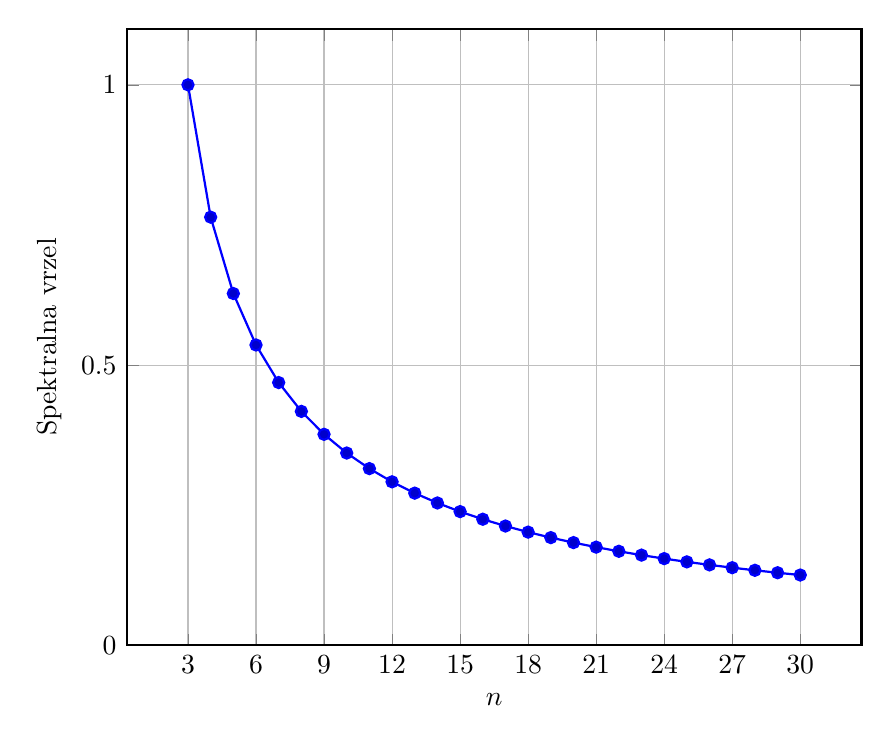
\begin{tikzpicture}
            \begin{axis}[
                    xlabel={$n$},
                    width=0.9\textwidth,
                    ylabel={Spektralna vrzel},
                    grid=major,
                    ymin=0, ymax=1.1,
                    xtick={3,6, 9,...,30},
                    ytick={0,0.5,1},
                    thick
                ]
                \addplot coordinates {
                    (3, 1.0)
                    (4, 0.7639320225002133)
                    (5, 0.6277186767309848)
                    (6, 0.5358983848622456)
                    (7, 0.4688711258507272)
                    (8, 0.41742430504416017)
                    (9, 0.3765246170202019)
                    (10, 0.34314575050761853)
                    (11, 0.31534156157350957)
                    (12, 0.2917960675006359)
                    (13, 0.2715838525995178)
                    (14, 0.2540333075851642)
                    (15, 0.23864417907084956)
                    (16, 0.2250356126078774)
                    (17, 0.21291218949664525)
                    (18, 0.20204102886728847)
                    (19, 0.19223593595585342)
                    (20, 0.18334617360803307)
                    (21, 0.1752483470938735)
                    (22, 0.16784043380076952)
                    (23, 0.1610373207469351)
                    (24, 0.1547674213348742)
                    (25, 0.1489700771813105)
                    (26, 0.14359353944898245)
                    (27, 0.13859338365492846)
                    (28, 0.13393125268149575)
                    (29, 0.12957385106060215)
                    (30, 0.12549213361245748)
                    };
            \end{axis}
        \end{tikzpicture}
        \caption{Graf spektralnih vrzeli ozkega grla za \(n\) od 1 do 30}
    \end{figure}
    Opazimo, da večji kot je \(n\), manjša je spektralna vrzel, prav tako kot je manjša Cheegerjeva konstanta (in bolj kot je izrazito ozko grlo). V primeru \(n=6\) dobimo drugo največjo lastno vrednost enako približno \(4{,}46\), iz česar sledi, da je spektralna vrzel približno \(0{,}54\).
\end{primer}
Nazadnje si oglejmo še primer naključnega grafa.
\begin{primer}[Naključen graf]\label{nakljucen-graf-lv}
    Izberemo isti graf kot v primeru \ref{nakljucen-graf-cheeger}. Njegova največja lastna vrednost je enaka \(5\), druga največja lastna vrednost pa je enaka približno \(3{,}50\). Spektralna vrzel je v tem primeru približno \(1{,}50\), kar je veliko več kot pri grafu ozkega grla.
\end{primer}

Računanje lastnih vrednosti regularnega grafa nam olajša tudi lastnost, da je njegova največja lastna vrednost enaka stopnji regularnosti.
\begin{izrek}[Največja lastna vrednost \(d\)-regularnega grafa]
    Največja lastna vrednost \(d\)-regularnega grafa je \(d\).
\end{izrek}

Izrek bomo nekoliko posplošili, kar nam bo kasneje v pomoč.
\begin{izrek}[Največja lastna vrednost matrike]\label{def-najvecja-lv}
    Naj bo \(A\) matrika z nenegativnimi vrednostmi, ki ima vsoto elementov v vsaki vrstici kvečjemu \(d\). Potem je največja lastna vrednost \(A\) manjša ali enaka \(d\).
\end{izrek}
\begin{dokaz}
    Naj bo \(v\) lastni vektor , ki ustreza lastni vrednosti \(\lambda\) matrike \(A\). Naj bo \(v_i\) največji element vektorja \(v\) in izračunajmo \(i\)-to vrstico produkta \(Av\).
    \begin{align*}
        (Av)_i = \sum_{k=1}^n A_{i,k}v_k \leq \sum_{k=1}^n A_{i,k}v_i \leq d\cdot v_i
    \end{align*}
\end{dokaz}
%\begin{dokaz}
%    Lastni vektor \(d\)-regularnega grafa \(G\) za lastno vrednost \(d\) je vedno vektor samih enic, saj ima vsaka vrstica sosednostne matrike natanko \(n\) enic.
%
%    Večje lastne vrednosti ne obstaja, saj so elementi sosednostne matrike samo \(0\) in \(1\). Če bi obstajala lastna vrednost \(\lambda > d\), potem si ogledamo največji element lastnega vektorja za to lastno vrednost, \(x\). Ker ima matrika natanko \(d\) enic v vsaki vrstici (in ostale vrednosti \(0\)), bi moralo obstajati \(d\) elementov vektorja, ki se skupaj sešteje v \(\lambda x\). Ker pa je vsak element manjši ali enak \(x\), imamo jih pa \(d\) lahko dosežemo kvečjemu \(d \times x\), torej večja lastna vrednost ne obstaja.
%\end{dokaz}
Torej če je graf regularen, potrebujemo le izračunati njegovo drugo največjo lastno vrednost. Vedno ima namreč lastno vrednost \(d\) za lastni vektor samih enic, dokazali pa smo, da večje lastne vrednosti ni.
\subsection{Cheegerjeva neenakost}
Opazili smo, da imata Cheegerjeva konstanta in spektralna vrzel podobno obnašanje. Definiciji nista enakovredni -- obstajajo grafi, pri katerih lahko z dodajanjem povezav znižamo spektralno vrzel (medtem, ko bo Cheegerjeva konstanta ne more postati nižja).

\begin{primer}[Dodajanje povezave poviša vrzel]
    % compute/edges_increase_gap.py
    Definiramo graf na šestih vozliščih s sosednostno matriko
    \begin{align*}
        \begin{bmatrix}
            0& 1& 1& 0& \color{red}\mathbf{1}& 1\\
            1& 0& 1& 1& 1& 1\\
            1& 1& 0& 1& 1& 1\\
            0& 1& 1& 0& 1& 1\\
            \color{red}\mathbf{1}& 1& 1& 1& 0& 0\\
            1& 1& 1& 1& 0& 0\\
        \end{bmatrix}.
    \end{align*}
    \begin{figure}[H]
        \centering
        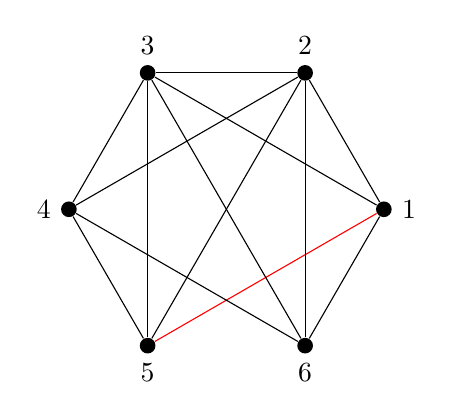
\begin{tikzpicture}
            \node[circle, fill=black, inner sep=2pt, label=right:1] (A) at (0.0: 2) {};
            \node[circle, fill=black, inner sep=2pt, label=above:2] (B) at (60.0: 2) {};
            \node[circle, fill=black, inner sep=2pt, label=above:3] (C) at (120.0: 2) {};
            \node[circle, fill=black, inner sep=2pt, label=left:4] (D) at (180.0: 2) {};
            \node[circle, fill=black, inner sep=2pt, label=below:5] (E) at (240.0: 2) {};
            \node[circle, fill=black, inner sep=2pt, label=below:6] (F) at (300.0: 2) {};
            \draw (B) -- (A);
            \draw (C) -- (A);
            \draw (C) -- (B);
            \draw (D) -- (B);
            \draw (D) -- (C);
            \draw[draw=red] (E) -- (A);
            \draw (E) -- (B);
            \draw (E) -- (C);
            \draw (E) -- (D);
            \draw (F) -- (A);
            \draw (F) -- (B);
            \draw (F) -- (C);
            \draw (F) -- (D);
        \end{tikzpicture}
    \end{figure}
    Spektralna vrzel grafa je približno \(2{,}37\), njegova Cheegerjeva konstanta pa približno \(2{,}33\). Če odstranimo povezavo med vozliščema \(1\) in \(5\), dobimo graf s spektralno vrzeljo približno \(2{,}43\) in Cheegerjevo konstanto \(2\). Tako smo poslabšali povezanost grafa, kar je razvidno iz nižje Cheegerjeve konstante, spektralno vrzel pa smo kljub temu povečali
\end{primer}

Kljub temu lahko povezavo med Cheegerjevo konstanto in spektralno vrzeljo vseeno formaliziramo \cite{chung-cheeger}.
\begin{izrek}[Cheegerjeva neenakost]\label{cheeger-neenakost}
    Naj bo \(G\) \(d\)-regularen graf. Potem velja 
    \begin{align*}
        \frac{1}{2}s(G) \leq c(G) \leq \sqrt{2ds(G)}
    \end{align*}
    oziroma
    \begin{align*}
        2c(G) \geq s(G) \geq \frac{c(G)^2}{2d}.
    \end{align*} 
\end{izrek}
Za dokaz izreka potrebujemo naslednjo lemo.
\begin{lema}\label{cheegerLema}
    Za poljubna \(a, b, c, d > 0\) velja
    \begin{align*}
        \frac{a+b}{c+d} \geq \min\left(\frac{a}{c}, \frac{b}{d}\right).
    \end{align*}
\end{lema}
\begin{dokaz}
    Začnemo z izrazom \(a+b\) in ga preoblikujemo.
    \begin{align*}
        a+b &= c\cdot\frac{a}{c} + d\cdot \frac{b}{d}
    \end{align*}
    Nato vpeljemo minimum in enostavno zaključimo dokaz.
    \begin{align*}
        a+b &\geq (c+d) \min\left(\frac{a}{c}, \frac{b}{d}\right)\\
        \frac{a+b}{c+d} &\geq \min\left(\frac{a}{c}, \frac{b}{d}\right)
    \end{align*}
\end{dokaz}
\begin{dokaz}[Dokaz Cheegerjeve neenakosti]
    Najprej dokažimo \(2c(G) \geq s(G)\). Naj bo \(S\subset V(G)\) množica, ki dosega minimum v definiciji Cheegerjeve konstante, torej \(0<\abs{S} \leq \abs{V(G)}/2\) in 
    \begin{align*}
        c(G) = \frac{\abs{\partial S}}{\abs{S }}.
    \end{align*}
    Spektralno vrzel poiščemo preko Rayleighovega kvocienta. Če je \(A\) sosednostna matrika grafa, je njen Rayleighov kvocient
    \begin{align*}
        R(A, v) = \frac{v^\top Av}{v^\top v}.
    \end{align*}
    Vemo, da je vektor samih enic lastni vektor sosednostne matrike za največjo lastno vrednost \(d\). Če želimo določiti drugo največjo lastno vrednost, poiščemo maksimum Rayleighovega kvocienta po vseh vektorjih, ki so pravokotni na vektor samih enic. Da dokažemo želeno neenakost, izberemo specifičen vektor \(v\) in izračunamo njegov Rayleighov kvocient. Druga največja lastna vrednost bo večja ali enaka od izračunanega kvocienta, spektralna vrzel pa zato manjša.

    Izberemo vektor \(v\) tako, da ima elemente enake \(\abs{S}^{-1}\) na indeksih, ki pripadajo elementom iz \(S\) ter ostale elemente (tiste, ki pripadajo indeksom za \(\overline S\)) enake \(-\abs{\overline S}^{-1}\). Ta vektor je pravokoten na vektor samih enic.

    Zdaj izračunamo Rayleighov kvocient. Najprej iračunamo pomen izraza \(v^tAv\) za sosednostne matrike.
    \begin{align*}
        Av = \left(\sum_{j=1}^{\abs{V(G)}} v_j \cdot A_{i,j}\right)_{i=1}^{\abs{V(G)}}\\
        v^\top Av = \sum_{i=1}^{\abs{V(G)}} \sum_{j=1}^{\abs{V(G)}} v_i v_j A_{i,j} = \sum_{i\sim j} v_i v_j\\
    \end{align*}
    Ta izraz nato vstavimo v definicijo Rayleighovega kvoceinta
    \begin{align*}
        R(A, v) &= \frac{\sum_{i\sim j} v_i v_j}{\sum_{i=1}^{\abs{V(G)}}v_i^2}
    \end{align*}
    Z enostavnimi operacijami poenostavimo izraz.
    \begin{align*}
        R(A,v) &= \frac{\sum_{i\sim j} v_i^2 + v_j^2 - \left(v_i - v_j\right)^2}{2 \sum_{i=1}^{\abs{V(G)}}v_i^2}\\
        &= \frac{\sum_{i\sim j} v_i^2}{\sum_{i=1}^{\abs{V(G)}}v_i^2} - \frac{\sum_{i\sim j}\left(v_i - v_j\right)^2}{2 \sum_{i=1}^{\abs{V(G)}}v_i^2}
    \end{align*}
    S pomočjo \(d\)-regularnosti lahko poenostavimo levi člen, desni člen pa lahko poenostavimo zaradi izbire \(v\) -- elementi vektorja, ki pripadajo \(S\) imajo namreč enake vrednosti, torej je njihova razlika enaka nič; enako velja za elemente, ki pripadajo \(\overline{S}\).
    \begin{align*}
        R(A, v) &= \frac{d\cdot \sum_{i=1}^{\abs{V(G)}}v_i^2}{\sum_{i=1}^{\abs{V(G)}}v_i^2} -  \frac{2\cdot \sum_{i\in S \land j \in \overline S}\left(v_i - v_j\right)^2}{2 \sum_{i=1}^{\abs{V(G)}}v_i^2}
    \end{align*}
    V izraz vstavimo definicijo \(v\) in dokaz dokončamo z enostavnim računom.
    \begin{align*}
        R(A, v) &= d - \frac{\abs{\partial S} \cdot \left(\frac{1}{\abs{S}} + \frac{1}{\abs{\overline S}}\right)^2}{\abs{S} \frac{1}{\abs{S}^2} + \abs{\overline S} \frac{1}{\abs{\overline S}^2}}\\
        &= d - \abs{\partial S}\left(\frac{1}{\abs{S}} + \frac{1}{\abs{\overline S}}\right) \\ 
        &= d - \frac{\abs{\partial S}}{\abs{S}}\frac{\left(\abs{S} + \abs{\overline S}\right)}{\abs{\overline S}}\\
        &= d- c(G) \frac{V(G)}{\abs{\overline S}}\\
        &\geq d - 2c(G)
    \end{align*}
    Torej velja
    \begin{align*}
        \lambda_2 \geq R(A,v) \geq d-2c(G),\\
        2c(G) \geq d-\lambda_2 = s(G).
    \end{align*}

    % file:///home/tadej/library/math/magistrska/cheeger_chung.pdf
    Zdaj dokažemo še drugo neenakost, \(s(G) \geq \frac{c(G)^2}{2d}\). Podobno kot v Fiedlerjevem algoritmu bomo s pomočjo lastnega vektorja, ki ustreza drugi največji lastni vrednosti, konstruirali particijo grafa.

    Naj bo \(v\) lastni vektor za drugo največjo lastno vrednost, \(\lambda_2\). Brez škode za splošnost preuredimo vozlišča grafa tako, da je \(v_i \geq v_j\) za \(i < j\). Definiramo množico \(S_i = \{v_1, \ldots, v_i\}\) in 
    \begin{align*}
        \alpha(G) = \min_{1\leq i \leq V(G)/2} \frac{\abs{\partial S_i}}{\abs{S_i}}.
    \end{align*}
    Očitno velja \(h(G) \leq \alpha(G)\).

    Definirajmo \(r=\floor{V(G)/2}\) in vektorja \(v^+\) in \(v^-\) kot
    \begin{align*}
        v^+_i = \begin{cases}
            v_i - v_r & v_i \geq v_r \\
            0 & v_i < v_r
        \end{cases}\\
        v^-_i = \begin{cases}
            v_r - v_i & v_i \leq v_r \\
            0 & v_i > v_r
        \end{cases}.
    \end{align*}
    Predpostavimo, da velja \(R(A, v^+) \geq R(A, v^-)\); če to ne drži, lastni vektor \(v\) pomnožimo z \(-1\). Izbrali smo \(r\) tako, da imata vektorja \(v^+\) in \(v^-\) kvečjemu \(r\) pozitivnih elementov. Ta lastnost se ohrani, če zamenjamo predznake v vektorju \(v\), kot zahteva predpostavka. Vozlišča, ki pripadajo pozitivnim elementom \(v^+\), bomo uporabili pri vpeljavi \(\alpha(G)\), ki pa zahteva podgraf velikosti največ \(r\). Predpostavko lahko zapišemo tudi drugače:
    \begin{align}\label{eq:cheegerPredpostavka}
        \frac{\sum_{i\sim j}(v^+_i - v^+_j)^2}{2\sum_{i=1}^{\abs{V(G)}} (v^+_i)^2} \leq \frac{\sum_{i\sim j} (v^-_i - v^-_j)^2}{2\sum_{i=1}^{\abs{V(G)}} (v^-_i)^2} 
    \end{align}
    % Ali napišem da primer če je v+ ali v- = 0 je trivialno

    Podobno kot v prvem delu dokaza preko Rayleighovega kvocienta izrazimo spektralno vrzel.
    \begin{align*}
        s(G) &= d-\lambda_2 \\ 
        &= \frac{\sum_{i\sim j}(v_i - v_j)^2}{2\sum_{i=1}^{\abs{V(G)}} v_i^2}
    \end{align*}
    
    Ker je \(v\) pravokoten na največji lastni vektor, vektor samih enic, velja \(\sum_i v_i = 0\). Tako lahko povečamo imenovalec kvocienta:
    \begin{align*}
        \sum_{i=1}^{\abs{V(G)}} v_i^2 = \min_{c\in \R} \sum_{i=1}^{\abs{V(G)}} (v_i - c)^2 \leq \sum_{i=1}^{\abs{V(G)}} (v_i - v_r)^2\\
        \frac{\sum_{i\sim j}(v_i - v_j)^2}{2\sum_{i=1}^{\abs{V(G)}} v_i^2} \geq \frac{\sum_{i\sim j}(v_i - v_j)^2}{2\sum_{i=1}^{\abs{V(G)}} (v_i-v_r)^2}
    \end{align*}
    Imenovalec lahko prepišemo z uporabo \(v^+\) in \(v^-\)
    \begin{align*}
        \frac{\sum_{i\sim j}(v_i - v_j)^2}{2\sum_{i=1}^{\abs{V(G)}} v_i^2} \geq \frac{\sum_{i\sim j}(v_i - v_j)^2}{2\sum_{i=1}^{\abs{V(G)}} (v_i-v_r)^2} = \frac{\sum_{i\sim j}(v_i - v_j)^2}{2\sum_{i=1}^{\abs{V(G)}} (v^+_i)^2 + 2\sum_{i=1}^{\abs{V(G)}} (v^-_i)^2}.
    \end{align*}
    
    Sedaj pomanjšamo števec \(\sum_{i\sim j}(v_i - v_j)^2\). Če sta \(v_i\) in \(v_j\) oba večja od \(v_r\), potem velja
    \begin{align*}
        (v_i - v_j)^2 = (v^+_i - v^+_j)^2 + (v^-_i - v^-_j)^2.
    \end{align*}
    Enako velja, če sta oba manjša od \(v_r\). Z enostavnim računom dobimo podoben rezultat v primeru, da velja \(v_j \leq v_r \leq v_i\).
    \begin{align*}
        0 \geq (v_r - v_i)(v_r - v_j)\\
        0 \geq v_r^2 - v_r v_i - v_r v_j + v_i v_j \\
        -2 v_i v_j \geq 2 v_r^2 - 2 v_r v_i - 2 v_r v_j \\
        v_i^2 - 2v_i v_j + v_j^2 \geq (v_r^2 - 2v_r v_i + v_i^2) + (v_r^2 - 2v_r v_j + v_j^2) \\ 
        (v_i - v_j)^2 \geq (v_i - v_r -0)^2 + (0 + v_j - v_r)^2 \\
        (v_i - v_j)^2 \geq  (v^+_i - v^+_j)^2 + (v^-_i - v^-_j)^2
    \end{align*}
    Enako velja v primeru \(v_i \leq v_r \leq v_j\), torej je
    \begin{align*}
        s(G) &\geq \frac{\sum_{i\sim j}(v_i - v_j)^2}{2\sum_{i=1}^{\abs{V(G)}} (v^+_i)^2 + 2\sum_{i=1}^{\abs{V(G)}} (v^-_i)^2}\\
        &\geq \frac{\sum_{i\sim j}(v^+_i - v^+_j)^2 + (v^-_i - v^-_j)^2}{2\sum_{i=1}^{\abs{V(G)}} (v^+_i)^2 + 2\sum_{i=1}^{\abs{V(G)}} (v^-_i)^2}
    \end{align*}
    
    Zgornjo neenakost lahko, s pomočjo predpostavke \eqref{eq:cheegerPredpostavka} in leme \ref{cheegerLema} spremenimo v

    \begin{align*}
        s(G) \geq  \frac{\sum_{i\sim j}(v^+_i - v^+_j)^2}{2\sum_{i=1}^{\abs{V(G)}} (v^+_i)^2}.
    \end{align*}
    Od tod sledi
    \begin{align*}
        s(G) &\geq  \frac{\sum_{i\sim j}(v^+_i - v^+_j)^2}{2\sum_{i=1}^{\abs{V(G)}} (v^+_i)^2} \frac{\sum_{i\sim j}(v^+_i + v^+_j)^2}{\sum_{i\sim j}(v^+_i + v^+_j)^2}\\
        &= \frac{\sum_{i\sim j}(v^+_i - v^+_j)^2}{2\sum_{i=1}^{\abs{V(G)}} (v^+_i)^2} \frac{\sum_{i\sim j}(v^+_i + v^+_j)^2}{\sum_{i\sim j}(v^+_i)^2 + (v^+_j)^2 + 2v^+_i v^+_j}\\
        &= \frac{\sum_{i\sim j}(v^+_i - v^+_j)^2}{2\sum_{i=1}^{\abs{V(G)}} (v^+_i)^2} \frac{\sum_{i\sim j}(v^+_i + v^+_j)^2}{2d\sum_{i=1}^{\abs{V(G)}} (v^+_i)^2 + 2\sum_{i\sim j}v^+_i v^+_j}
    \end{align*}
    Uporabimo Cauchy-Schwarzovo neenakost ločeno na števcu in na delu imenovalca.
    \begin{align*}
        s(G) &\geq  \frac{\left(\sum_{i\sim j}(v^+_i - v^+_j)(v^+_i + v^+_j)\right)^2}{2\sum_{i=1}^{\abs{V(G)}} (v^+_i)^2\left(2d\sum_{i=1}^{\abs{V(G)}} (v^+_i)^2 + 2\sqrt{\sum_{i\sim j}(v^+_i)^2 \sum_{i\sim j} (v^+_j)^2}\right)}
    \end{align*}
    Poenostavimo izraz v imenovalcu
    \begin{align*}
        s(G) &\geq \frac{\left(\sum_{i\sim j}\abs{(v^+_i)^2 - (v^+_j)^2} \right)^2}{2\sum_{i=1}^{\abs{V(G)}} (v^+_i)^2 \left(2d\sum_{i=1}^{\abs{V(G)}} (v^+_i)^2 + 2d \sum_{i=1}^{\abs{V(G)}}(v^+_i)^2 \right)}\\
        &= \frac{\left(\sum_{i\sim j}\abs{(v^+_i)^2 - (v^+_j)^2} \right)^2}{8d\left(\sum_{i=1}^{\abs{V(G)}} (v^+_i)^2\right)^2}
    \end{align*}
    Ker je graf neusmerjen, vemo, da če imamo povezavo \(i\sim j\), imamo tudi \(j\sim i\). V števcu torej vsako povezavo štejemo dvakrat.
    \begin{align*}
        s(G) &\geq \frac{\left(2\sum_{i\sim j \land i< j}(v^+_i)^2 - (v^+_j)^2 \right)^2}{8d\left(\sum_{i=1}^{\abs{V(G)}} (v^+_i)^2\right)^2} \\
        &= \frac{\left(\sum_{i\sim j \land i< j}(v^+_i)^2 - (v^+_j)^2 \right)^2}{2d\left(\sum_{i=1}^{\abs{V(G)}} (v^+_i)^2\right)^2}
    \end{align*}
    Vsak sumand \((v^+_i)^2 - (v^+_j)^2\) lahko teleskopsko razpišemo kot
    \begin{align*}
        (v^+_i)^2 &- (v^+_{i+1})^2\\
        + (v^+_{i+1})^2 &- (v^+_{i+2})^2\\
        + &\cdots\\
        + (v^+_{j-1})^2 &- (v^+_{j})^2,
    \end{align*}
    da dobimo
    \begin{align*}
        s(G) &\geq \frac{\left(\sum_{i=1}^{\abs{V(G)}}\abs{\partial S_i}\left((v^+_i)^2 - (v^+_{i+1})^2\right) \right)^2}{2d\left(\sum_{i=1}^{\abs{V(G)}} (v^+_i)^2\right)^2}\\
        &=\frac{\left(\sum_{i=1}^{r}\abs{\partial S_i}\left((v^+_i)^2 - (v^+_{i+1})^2\right) \right)^2}{2d\left(\sum_{i=1}^{r} (v^+_i)^2\right)^2}
    \end{align*}
    Po definiciji za vsak \(i\leq r\) velja \(\abs{\partial S_i} \geq \abs{S_i} \alpha(G)\).
    \begin{align*}
        s(G) &\geq \frac{\left(\sum_{i=1}^{r} \abs{S_i} \alpha(G)\left((v^+_i)^2 - (v^+_{i+1})^2\right) \right)^2}{2d\left(\sum_{i=1}^{r} (v^+_i)^2\right)^2}
    \end{align*}
    Dokaz lahko zaključimo z enostavnim računom.
    \begin{align*}
        s(G) &\geq \frac{\alpha(G)^2}{2d} \frac{\left(\sum_{i=1}^{r} \abs{S_i}\left((v^+_i)^2 - (v^+_{i+1})^2\right) \right)^2}{\left(\sum_{i=1}^{r} (v^+_i)^2\right)^2}\\
        &= \frac{\alpha(G)^2}{2d} \frac{\left(\sum_{i=1}^{r} i\cdot (v^+_i)^2 - \sum_{i=1}^{r} (i-1) \cdot (v^+_{i})^2 \right)^2}{\left(\sum_{i=1}^{r} (v^+_i)^2\right)^2}\\
        &= \frac{\alpha(G)^2}{2d} \frac{\left(\sum_{i=1}^{r} i\cdot (v^+_i)^2 - \sum_{i=1}^{r} (i-1) \cdot (v^+_{i})^2 \right)^2}{\left(\sum_{i=1}^{r} (v^+_i)^2\right)^2}\\
        &= \frac{\alpha(G)^2}{2d} \frac{\left(\sum_{i=1}^{r} \cdot (v^+_i)^2 \right)^2}{\left(\sum_{i=1}^{r} (v^+_i)^2\right)^2}\\
        &= \frac{\alpha(G)^2}{2d}\\
    \end{align*}
    Tako dobimo
    \begin{align*}
        s(G) \geq \frac{\alpha(G)^2}{2d} \geq \frac{h(G)^2}{2d}.
    \end{align*}
\end{dokaz}
\subsection{Alon-Boppanov izrek}
Naša prvotna motivacija je bila iskanje grafov, ki so čim bolje povezani. Cheegerjeva neenakost upraviči, da poskušamo maksimizirati spektralno vrzel oziroma minimizirati drugo največjo lastno vrednost. Izkaže pa se, da druga največja lastna vrednost ne more biti poljubno majhna, kar opisuje Alon-Boppanov izrek. Izrek, kot ga je dokazal Alon omeji drugo največjo lastno vrednost \(d\)-regularnega grafa. Če je \(\lambda_2\) druga največja lastna vrednost \(d\)-regularnega grafa in obstajata dve povezavi, katerih krajišča sta med seboj oddaljeni vsaj \(2(k+1)\) (oziroma najkrajša pot v grafu med njima je \(2(k+1)\)), potem se Alon-Boppanov \cite{alon-boppana-original} izrek glasi 
\begin{align*}
    \lambda_2 \geq 2\sqrt{d-1} - \frac{\sqrt{d-1}}{2(k+1)^2}.
\end{align*}
Vidimo, da bolj kot povečamo število vozlišč v grafu, večji je lahko \(k\). Nas zanima prav različica izreka, ki opisuje asimptotično obnašanje druge največje lastne vrednosti, ko število vozlišč grafa raste proti neskončnosti. Priročno bo tudi, da namesto druge največje lastne vrednosti gledamo po absolutni vrednosti največjo netrivialno lastno vrednost, izrek bi pa sicer deloval tudi brez tega. Kot trivialno lastno vrednost štejemo \(d\), ker je vedno prisotna v vseh \(d\)-regularnih grafih, prav tako pa \(-d\) pri dvodelnih \(d\)-regularnih grafih \cite{lps-ramanujan}.

\begin{izrek}[Alon-Boppanova meja]
    \label{alon-boppanova-meja-izrek}
    Naj bo \(\{G_n\}\) neskončna družina \(d\)-regularnih grafov, kjer ima \(G_n\) \(n\) vozlišč in \(\lambda(G)\) absolutna vrednost največje netrivialne lastne vrednosti. Potem velja
    \begin{align*}
        \lim_{n\to\infty} \lambda(G_n) \geq 2\sqrt{d-1}.
    \end{align*}
\end{izrek}
V dokazu bomo velikost lastnih vrednosti ocenili s številom sprehodov določene dolžine v grafu. Sprehodi, v poljubnem \(d\)-regularnem grafu \(G\) pa so tesno povezani s sprehodi v \(d\)-regularnem neskončnem drevesu. Vsako vozlišče lahko uporabimo kot koren drevesa, torej si oglejmo sprehode iz korena ter jih primerjamo s sprehodi iz poljubnega vozlišča \(x\) grafa. Vsakemu vozlišču drevesa bomo dodelili (ne nujno unikatno) oznako, ki določa, kateremu vozlišču v \(G\) pripada. Koren drevesa poimenujemo \(x\), njegove sosede pa poimenujemo enolično po sosedih \(x\) v \(G\). Ta proces induktivno ponavljamo ter otroke vozlišča \(v\) v drevesu poimenujemo po sosedih vozlišča \(v\) v \(G\), ki niso enaki staršu \(v\) v drevesu. Če v tako označenem drevesu naredimo sprehod, bo zaporedje obiskanih vozlišč opisovalo sprehod v \(G\). Bolj specifično, vsak sprehod iz korena \(x\) do korena \(x\) v drevesu enolično določa tudi sprehod iz \(x\) do \(x\) v \(G\), ne pa nujno tudi obratno. Vsi takšni sprehodi v drevesu bodo sode dolžine, očitno pa niso vsi cikli vseh grafov sodi. Število sprehodov dolžine \(l\) v drevesu, ki se začnejo in končajo v istem vozlišču, bomo poimenovali \(\rho(l)\). Če pa štejemo le sprehode dolžine \(l\), ki se začnejo in končajo v istem vozlišču, med sprehodom pa, razen na krajiščih, nikoli ne obiščejo tega vozlišča, pa to označimo \(\rho'(l)\). Seveda je \(\rho(l)\geq \rho'(l)\), oba pa sta manjša od števila sprehodov v grafu \(G\) dolžine \(l\) iz poljubnega vozlišča do samega sebe. Poleg tega vedno velja \(\rho(2l+1)=0\). Za dokaz Alon-Boppanove meje moramo izračunati \(\rho'(l)\), saj nam bo to omogočilo omejitev velikosti lastnih vrednosti \cite{polatajko}.
\begin{lema}[Število sprehodov v drevesu]\label{alon:drevesa-meja}
    V \(d\)-regularnem drevesu \(T\) je število sprehodov dolžine \(2l\), ki se začnejo in končajo v istem vozlišču ter ga med potjo ne obiščejo več, enako
    \begin{align*}
        \frac{1}{l}\binom{2l-2}{l-1}d(d-1)^{l-1} = \rho'(2l).
    \end{align*}
\end{lema}
\begin{dokaz}
    Oglejmo si sprehod dolžine \(2l\), ki se začne v korenu drevesa. Vsak tak sprehod skupaj naredi \(l\) korakov iz vozlišča k njegovemu otroku ter \(l\) korakov iz vozlišča proti njegovemu staršu. 
    
    Najprej si oglejmo zaporedje teh korakov. Vsak korak proti potomcu predstavimo s \(+1\), vsak korak proti staršu pa z \(-1\). Če izpustimo prvi in zadnji korak (saj sta vedno \(+1\) in \(-1\)), imamo \(l-1\) vrednosti \(+1\) in \(l-1\) vrednosti \(-1\). Vseh takih zaporedij je
    \begin{align*}
        \binom{2(l-1)}{l-1}.
    \end{align*}
    Ker se pred koncem sprehoda ne želimo vrniti v koren, mora biti ob vsakem dodanem številu seštevek vseh števil nenegativen. Oglejmo si zaporedja ki prekršijo to pravilo. Za taka zaporedja \((a_1, \ldots, a_{2l-2})\) obstaja nek najmanjši \(k\), da je \(a_{2k+1}=-1\) in \(\sum_{i=1}^{2k} a_i = 0\). Definirajmo funkcijo \(f\) na takšnih zaporedjih, ki spremeni predznak prvih \(2k+1\) elementov, preostale elemente pa pusti nespremenjene. Ker je med prvimi \(2k\) elementi enako število vrednosti \(+1\) in \(-1\), ostane uravnoteženost nespremenjena tudi po zamenjavi predznakov. Ker je število \(+1\) in \(-1\) enako tudi v celotnem zaporedju dolžine \(2l-2\), pomeni, da je število \(+1\) in \(-1\) v prvotnem zaporedju enako tudi na zadnjih \(2l-2-2k\) elementih; ker pa smo zamenjali element \(a_{2k+1}\) iz \(-1\) na \(+1\) bo v transformiranem zaporedju \(f(a)\) zato na zadnjih \(2l-2-2k\) elementih \(l-2-k\) elementov \(-1\) in \(l-k\) elementov \(+1\). Združimo vse ugotovitve: v \(f(a)\) je natanko \(l\) elementov \(+1\) in \(l-2\) elementov \(-1\). 
    
    Trdimo, da je \(f\) bijekcija med zaporedji, ki imajo nekje negativno delno vsoto, ter zaporedji z \(l\) vrednostmi \(+1\) in \(l-2\) vrednostmi \(-1\). Inverz funkcije \(f\) poišče prvi element, kjer je delna vsota enaka \(+1\), in zamenja predznake tega elementa ter vseh elementov pred njim. Dokažimo, da ta operacija res definira inverz. Če imamo dva zaporedja \(x\) in \(y\) z \(f(x)=f(y)\), ta inverz očitno pokaže, da velja \(x=y\), torej je \(f\) injektivna. Za surjektivnost opazimo, da imajo zaporedja iz kodomene več elementov \(+1\) kot \(-1\). Zato mora obstajati vsaj ena delna vsota, ki je enaka \(+1\), in lahko uporabimo inverz. Zaporedij iz kodomene je \(\binom{2l-2}{l}\), torej je toliko tudi zaporedij, ki prekršijo pravilo, da je delna vsota vedno nenegativna.
    
    Sedaj izračunajmo število zaporedij, ki ustrezajo prvotnim zahtevam (torej zaporedij, ki nimajo negativne delne vsote). To storimo tako, da od števila vseh zaporedij dolžine \(2l-2\) z enakim številom \(+1\) in \(-1\) odštejemo število teh, z negativno delno vsoto. 
    \begin{align*}
        &\binom{2l-2}{l-1} - \binom{2l-2}{l}\\
        =& \frac{(2l-2)!}{(l-1)!(l-1)!} - \frac{(2l-2)!}{l!(l-2)!}\\
        =& \frac{(2l-2)!}{(l-1)!(l-2)!}\left(\frac{1}{l-1} - \frac1l \right)\\
        =& \frac{(2l-2)!}{(l-1)!(l-2)!}\frac{1}{l(l-1)}\\
        =& \frac{1}{l}\binom{2l-2}{l-1}
    \end{align*}
    
    Pri vsakem koraku k potomcu nimamo le ene izbire. Prvi korak lahko vodi k kateremu koli izmed \(d\) potomcev. Pri vsakem od naslednjih \(l-1\) korakov proti potomcem imamo \(d-1\) možnih izbir. Da dobimo skupno število vseh sprehodov le zmnožimo ta števila skupaj
    \begin{align*}
        \rho'(2l) = \frac{1}{l}\binom{2l-2}{l-1} d (d-1)^{l-1}.
    \end{align*}
\end{dokaz}
\begin{dokaz}[Dokaz Alon-Boppanovega izreka]
    Naj bo \(A_n\) sosednostna matrika grafa \(G_n\). Potem \((i,j)\)-ti element matrike \(A_n^k\) predstavlja število poti dolžine \(l\) med vozliščema \(i\) in \(j\); označimo ga z \(\delta_{(i,j)}(l)\). Če so lastne vrednosti matrike \(A_n\) enake \(d=\lambda_1\geq \lambda_2 \geq \cdots \geq \lambda_n\), potem so lastne vrednosti matrike \(A_n^l\) enake \(\lambda_j^l\) za \(1\leq j \leq n\). Ker je sled matrike neodvisen od baze, lahko  matriko napišemo v lastni bazi in vidimo
    \begin{align*}
        \sum_{j=1}^n \lambda_j^l = \sum_{j=1}^n \delta_{(j, j)}(l).
    \end{align*}
    Če je \(\rho(l)\) število poti dolžine \(l\) iz vozlišča do samega sebe v \(d\)-regularnem drevesu, \(\rho'(l)\) pa število poti dolžine \(l\) iz vozlišča do samega sebe, ki ne obiščejo izvornega vozlišča predčasno, velja, kot smo omenili v orisu dokaza, \(\rho'(l) \leq \rho(l)\leq \delta_{(j,j)}(l)\) neodvisno od \(j\). Zato lahko poenostavimo izraz v
    \begin{align*}
        \sum_{j=1}^n \lambda_j^l \geq n \rho'(l).
    \end{align*}
    Če si ogledamo le poti sode dolžine in upoštevamo, da so vse lastne vrednosti razen največje (\(d\)) in morda najmanjše (ki je po absolutni vrednosti kvečjemu \(d\)) manjše od \(\lambda(G)\), dobimo
    \begin{align*}
        (n-2)\lambda(G)^{2l} + 2d^{2l} \geq \sum_{j=1}^n \lambda_j^l.
    \end{align*}
    Z uporabo prejšnje neenakosti lahko izraz poenostavimo.
    \begin{align*}
        (n-2)\lambda(G)^{2l} &\geq n\rho'(2l) - 2d^{2l}\\
        \lambda(G)^{2l} &\geq \frac{n}{n-2}\rho'(2l) - \frac{2d^{2l}}{n-2}\\
        \lambda(G)^{2l} &\geq \rho'(2l) - \frac{2d^{2l}}{n-2}
    \end{align*}
    Sedaj na izrazu uporabimo lemo \ref{alon:drevesa-meja}.
    \begin{align*}
        \lambda(G)^{2l} &\geq \frac{1}{l}\binom{2l-2}{l-1}d(d-1)^{l-1} - \frac{2d^{2l}}{n-2} \\
        \lambda(G)^{2l} &\geq \frac{1}{l}\binom{2l-2}{l-1}(d-1)^{l} - \frac{2d^{2l}}{n-2}
    \end{align*}
    V izraz vpeljemo limito.
    \begin{align*}
        \lim_{n\to\infty} \lambda(G)^{2l} &\geq \frac{1}{l}\binom{2l-2}{l-1}(d-1)^{l}\\
        \lim_{n\to\infty} \lambda(G) &\geq \sqrt[2l]{\frac{1}{l}}\cdot \sqrt[2l]{\binom{2l-2}{l-1}}\cdot \sqrt[2l]{(d-1)^{l}}
    \end{align*}
    Neenakost velja za vse \(l\) torej velja tudi v limiti \(l\to\infty\). Ko poračunamo limite \cite{polatajko} dobimo
    \begin{align*}
        \lim_{n\to\infty} \lambda(G) \geq 1 \cdot 2 \cdot \sqrt{d-1}.
    \end{align*}
\end{dokaz}
\subsection{Ramanujanovi grafi}
Zdaj lahko definiramo Ramanujanove grafe. V uvodu smo povedali, da želimo visoko povezane grafe. Nato smo pokazali, da spektralna vrzel opisuje, kako močno je graf povezan. Nazadnje smo dokazali, da je za neskončno družino grafov \(\lambda(G)\) (in posledično tudi druga največja lastna vrednost, ki določa spektralno vrzel) v limiti kvečjemu \(2\sqrt{d-1}\). Ramanujanovi grafi imajo \(\lambda(G)\) optimalen in, če imamo neskončno družino \(d\)-regularnih Ramanujanovih grafov, bo \(\lambda(G)\) v limiti natanko \(2\sqrt{d-1}\) in so na ta način optimalni glede na Alon-Boppanov izrek.

\begin{definicija}[Ramanujanov graf]
    Ramanujanov graf je \(d\)-regularen graf \(G\), za katerega velja
    \begin{align*}
        \lambda(G) \leq 2\sqrt{d-1}.
    \end{align*}
\end{definicija}

\begin{primer}[Polni grafi]
    Vsi polni grafi \(K_n\) so \((n-1)\)-regularni. Največja lastna vrednost \(K_n\) je \(n-1\), druga največja pa, kot smo izračunali v primeru \ref{polni-grafi-racun}, \(-1\). Torej je
    \begin{align*}
        \lambda(K_n) = 1 \leq 2\sqrt{n-2}
    \end{align*}
    in grafi so Ramanujanovi za vsak \(n>2\).
\end{primer}
Ta primer pokaže, da so Ramanujanovi grafi res dobro povezani. Graf namreč ne bi moral biti bolje povezan kot poln graf in polni grafi so Ramanujanovi. Kriterij za Ramanujanove grafe pa zahteva, da je graf dobro povezan glede na njegovo stopnjo regularnosti. Če je stopnja regularnosti manjša je tudi kriterij za povezanost manj strog. Poglejmo si ekstremen primer za cikle.
\begin{primer}[Cikli]
    Cikli so vedno \(2\)-regularni. V tem primeru definicija Ramanujanovega grafa zahteva, da je
    \begin{align*}
        \lambda(G) \leq 2.
    \end{align*}
    Ker pa je \(2\) največja lastna vrednost \(2\)-regularnih grafov, očitno druga največja lastna vrednost ne more biti večja. Torej so vsi cikli Ramanujanovi.
\end{primer}
% protiprimer iz uvoda
Zaključimo še z primeroma grafa ozkega grla in naključnega grafa.
\begin{primer}[Ozko grlo]
    V primeru \ref{ozko-grlo-lv} smo izračunali drugo največjo lastno vrednost grafa ozkega grla za primer \(n=5\); bila je približno \(4{,}46\). Ta vrednost je tudi največja netrivialna lastna vrednost. Ker je graf \(5\)-regularen, je pogoj, da je graf Ramanujanov to, da je ta lastna vrednost manjša ali enaka \(2\sqrt{5-1}\).
    \begin{align*}
       4{,}46 \approx \lambda(G) \not\leq 2\sqrt{5-1} = 4 
    \end{align*} 
    Ker to ne velja, graf ozkega grla ni Ramanujanov, kot smo pričakovali, saj je slabo povezan.
\end{primer}
\begin{primer}[Naključen graf]
    Izberemo enak graf, kot v primeru \ref{nakljucen-graf-lv}. Izračunali smo, da je njegova največja netrivialna lastna vrednost približno \(3{,}50\).
    \begin{align*}
        3{,}50 \approx \lambda(G) \leq 2\sqrt{5-1} = 4  
     \end{align*}
     Vidimo, da ta lastna vrednost ustreza pogoju za Ramanujanove grafe in graf je dobro povezan.
\end{primer}

\subsection{Konstante za grafe}
Ogledali si bomo nekaj konstant, ki jih lahko priredimo vsakemu grafu \cite{ramanujan-construction-book}. Ramanujanovi grafi nam poleg dobre povezanosti omogočajo tudi ocene za nekatere druge konstante.

\begin{definicija}[Kromatično število]
    Kromatično število \(\chi(G)\) grafa \(G\) je najmanjše število barv, ki jih priredimo vozliščem grafa \(G\), da nobeni dve sosednji vozlišči nista enake barve.
\end{definicija}
\begin{definicija}[Neodvisnostno število]
    Neodvisnostno število \(i(G)\) grafa \(G\) je velikost največje podmnožice vozlišč, v kateri si nobena dva vozlišča nista sosednja.
\end{definicija}

Oglejmo si, kako so te konstante povezane z drugo največjo lastno vrednostjo grafa.
% stran 31
\begin{izrek}
    Naj bo \(G\) \(d\)-regularen graf na \(n\) vozliščih, ki ni dvodelen. Potem velja
    \begin{align*}
        i(G) \leq \frac{n}{d} \lambda(G).
    \end{align*}
\end{izrek}
\begin{dokaz}
    Naj bo \(G=(V, E)\) graf in, kot v definiciji \(i\), naj bo \(F\subseteq V\) množica kardinalnosti \(i(G)\), v kateri nista nobena dva vozlišča sosednja.

    Vsakemu vozlišču določimo utež, podobno kot pri dokazu Cheegerjeve neenakosti \ref{cheeger-neenakost}.
    \begin{align*}
        v_j = \begin{cases}
            \abs{V-F} & j\in F \\
            -\abs{F} & j\not\in F
        \end{cases}
    \end{align*}
    Seštevek kvadratov elementov vektorja \(v\) lahko omejimo z uporabo neodvisnostnega števila.
    \begin{align*}
        \sum_{j\in V} v_j^2 &= \abs{F}\abs{V-F}^2 + \abs{V-F}\abs{F}^2 \\
                            &= \abs{F}\abs{V-F}(\abs{F}+\abs{V-F}) \\
                            &= \abs{F}\abs{V-F}n \\
                            &\leq i(G) n^2
    \end{align*}
    Izračunamo lahko še produkt \(v\) s sosednostno matriko \(A\).
    \begin{align*}
        (Av)_j = \sum_{k\sim j} v_k
    \end{align*}
    Če je \(j\in F\), potem vemo, da so vsi njegovi sosedi izven \(F\). Ker je \(d\)-regularen, pa je takih sosedov \(d\). Torej za tak \(j\) velja
    \begin{align*}
        (Av)_j = -d \abs{F} = -d\cdot i(G).
    \end{align*}
    Takih vozlišč \(j\) je pa ravno \(i(G)\). S tem lahko omejimo seštevek kvadratov produkta \(A v\).
    \begin{align*}
        \sum_{j\in V} (Av)_j^2 \geq d^2 i(G)^3
    \end{align*}
    Ker je seštevek \(\sum_{j\in V} v_j\) enak \(0\) vemo, da je vektor \(v\) pravokoten na vektor samih enic, ki je lastni vektor za lastno vrednost \(d\). Torej je razmerje \(\norm{A v} / \norm{ v} \leq \lambda(G)\). Če vstavimo izračunane norme dobimo
    \begin{align*}
        \frac{\norm{A v}}{\norm v} \leq \lambda(G) \\
        \norm{A v} \leq \lambda(G) \norm v
    \end{align*} 
    Da zaključimo dokaz le vstavimo prej-izračunano vrednost \(i(G)\) in izraz poenostavimo.
    \begin{align*}
        d^2 i(G)^3 \leq \lambda(G)^2 i(G) n^2\\
        i(G) \leq \frac{n}{d} \lambda(G)
    \end{align*}
\end{dokaz}

Oglejmo si še povezavo med kromatičnim številom in drugo največjo lastno vrednostjo grafa.
\begin{izrek}
    Naj bo \(G\) graf z \(n\) vozlišči. Potem velja
    \begin{align*}
        n \leq i(G)\cdot \chi(G).
    \end{align*}
\end{izrek}
\begin{dokaz}
    Naj bo \(V = V_1\cup V_2 \cup \cdots \cup V_{\chi(G)}\) barvanje grafa \(G\) z \(\chi(G)\) barvami. Po definiciji si vozlišča znotraj vsakega \(V_i\) niso sosedna, zato velja \(\abs{V_i} \leq i(G)\). Tako dobimo
    \begin{align*}
        n = \sum_{i=1}^{\chi(G)} \abs{V_i} \leq i(G) \chi(G).
    \end{align*}
\end{dokaz}
\begin{posledica}
    Za ne-dvodelen \(d\)-regularen graf \(G\) velja
    \begin{align*}
        \chi(G) \geq \frac{d}{\lambda(G)}.
    \end{align*}
    Če je graf Ramanujanov, potem velja
    \begin{align*}
        \chi(G) \geq \frac{d}{2\sqrt{d-1}} \approx \frac{\sqrt d}{2}.
    \end{align*}
\end{posledica}

Če poiščemo torej kakšen Ramanujanov graf, smo tudi poiskali graf z dovolj majhnim neodvisnostnim številom in dovolj velikim kromatičnim številom.